\section{Background}
\frame {
    \frametitle{Vector Boson Fusion (VBF)}

    \begin{columns}
        \begin{column}{0.5\textwidth}
            \begin{tikzpicture} \begin{feynman}
                \vertex (a);
                \vertex [right=of a] (b) {H};
                \vertex [above left=of a] (vb1);
                \vertex [below left=of a] (vb2);
                \vertex [left=of vb1] (q1i) {q};
                \vertex [left=of vb2] (q2i) {q};
                \vertex [above =of b] (q1f) {q};
                \vertex [below =of b] (q2f) {q};

                \diagram* {
                    (q1i) -- (vb1) -- (q1f),
                    (q2i) -- (vb2) -- (q2f), 
                    (vb1) -- [boson] (a) -- [boson] (vb2),
                    (a) -- [scalar] (b),
                };
            \end{feynman} \end{tikzpicture}

            \vspace{5mm}

            {\scriptsize
                Typical VBF tagging algorithms use the high invariant mass of the two VBF "signal" jets ($M_{jj}$),
                as well as their wide seperation in $\eta$ as an effective means of tagging them.

            }
        \end{column}
        \begin{column}{0.5\textwidth}
            VBF is the second highest Higgs production mechanism, but with a much cleaner signal than ggF
            %TODO: WHYYY is ggF not clean (maybe you don't need any pictures, but you should at least know for yourself... maybe you do need pictures though)

            \begin{figure}
                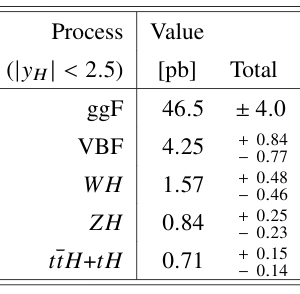
\includegraphics[width=\linewidth,height=0.5\textheight,keepaspectratio]{higgs_production_modes.png}
                \caption{source - arXiv:1909.02845 [hep-ex] }
            \end{figure}
        \end{column}
    \end{columns}
}

% Show your table of how common this is (~20%)
\displaytwo{VBF is a Two-Jet Process... But Not Always}
    {
        Due to unsuppressed pileup and radiation effects,
        there can often be more than just the two VBF signal jets present.
    }
    {remote/jet_counts/jet_counts_30GeV.pdf}
    {remote/figures/fig_eventCounts_sig.pdf}

\frame {
    \frametitle{The Complication of Many Jets}
    \begin{columns}
        \begin{column}{0.5\textwidth}
            \underline{\large Initial State Radiation (ISR)} \\ \vspace{5mm}
            \resizebox{0.95\textwidth}{!}{\begin{tikzpicture} \begin{feynman}
                \vertex (a);
                \vertex [right=of a] (b) {H};
                \vertex [above left=of a] (vb1);
                \vertex [below left=of a] (vb2);
                \vertex [left=of vb1] (q1i) {q};
                \vertex [below left=of vb2] (q2k);
                \vertex [left=of q2k] (q2i) {q};
                \vertex [above =of b] (q1f) {q};
                \vertex [below =of b] (q2f) {q};
                \vertex [below =of q2f] (g) {g (ISR)};

                \diagram* {
                    (q1i) -- (vb1) -- (q1f),
                    (q2i) -- (q2k) -- (vb2) -- (q2f),
                    (q2k) --[gluon] (g),
                    (vb1) -- [boson] (a) -- [boson] (vb2),
                    (a) -- [scalar] (b),
                };
            \end{feynman} \end{tikzpicture}}
        \end{column}
        \begin{column}{0.4\textwidth}
            \underline{\large Final State Radiation (FSR)} \\ \vspace{5mm}
            \resizebox{0.95\textwidth}{!}{\begin{tikzpicture} \begin{feynman}
                \vertex (a);
                \vertex [right=of a] (b) {H};
                \vertex [above left=of a] (vb1);
                \vertex [below left=of a] (vb2);
                \vertex [left=of vb1] (q1i) {q};
                \vertex [left=of vb2] (q2i) {q};
                \vertex [below right=of vb2] (q2k);
                \vertex [above =of b] (q1f) {q};
                \vertex [below =of b] (q2f) {q};
                \vertex [below =of q2f] (g) {g (FSR)};

                \diagram* {
                    (q1i) -- (vb1) -- (q1f),
                    (q2i) -- (vb2) -- (q2k) -- (q2f), 
                    (q2k) --[gluon] (g),
                    (vb1) -- [boson] (a) -- [boson] (vb2),
                    (a) -- [scalar] (b),
                };
            \end{feynman} \end{tikzpicture}}
        \end{column}
    \end{columns}
}

\frame {
    \frametitle{How is VBF Currently Handled?}
    \begin{columns}
        \begin{column}{0.7\textwidth}
            VBF$\rightarrow$H$\rightarrow$invisible

            {\tiny
            (source - Phys. Lett. B 793 (2019) 499)
            \begin{quote}
                 - a leading jet with $p_T$ > 80 GeV, \\
                 - a subleading jet with $p_T$ > 50 GeV, \\
                 - no additional jets with $p_T$ > 25 GeV, \\
            \end{quote}
            }
        \end{column}
        \begin{column}{0.3\textwidth}
            \resizebox{0.7\textwidth}{!}{\begin{tikzpicture} \begin{feynman}
                \vertex (a);
                \vertex [right=of a] (b) {H};
                \vertex [above right=of b] (inv1) {$\chi$};
                \vertex [below right=of b] (inv2) {$\bar \chi$};
                \vertex [above left=of a] (vb1);
                \vertex [below left=of a] (vb2);
                \vertex [left=of vb1] (q1i) {q};
                \vertex [left=of vb2] (q2i) {q};
                \vertex [above=of inv1] (q1f) {q};
                \vertex [below=of inv2] (q2f) {q};

                \diagram* {
                    (q1i) -- (vb1) -- (q1f),
                    (q2i) -- (vb2) -- (q2f), 
                    (vb1) -- [boson] (a) -- [boson] (vb2),
                    (a) -- [scalar] (b) --[boson] { (inv1), (inv2)}
                };
            \end{feynman} \end{tikzpicture}}
        \end{column}
    \end{columns}
    \vspace{\fill}
    \begin{columns}
        \begin{column}{0.7\textwidth}
            VBF$\rightarrow$H$\rightarrow$diphoton

            {\tiny
            (source - DOI: 10.1103/PhysRevD.98.052005)
            \begin{quote}
                Events are required to contain at least two hadronic jets,
                and the selections applied are based on the two leading jets $(j_1, j_2)$ in the event.
            \end{quote}
            }
        \end{column}
        \begin{column}{0.3\textwidth}
            \resizebox{0.7\textwidth}{!}{\begin{tikzpicture} \begin{feynman}
                \vertex (a);
                \vertex [right=of a] (b) {H};
                \vertex [above right=of b] (gam1) {$\gamma$};
                \vertex [below right=of b] (gam2) {$\gamma$};
                \vertex [above left=of a] (vb1);
                \vertex [below left=of a] (vb2);
                \vertex [left=of vb1] (q1i) {q};
                \vertex [left=of vb2] (q2i) {q};
                \vertex [above=of gam1] (q1f) {q};
                \vertex [below=of gam2] (q2f) {q};

                \diagram* {
                    (q1i) -- (vb1) -- (q1f),
                    (q2i) -- (vb2) -- (q2f), 
                    (vb1) -- [boson] (a) -- [boson] (vb2),
                    (a) -- [scalar] (b) --[boson] { (gam1), (gam2)}
                };
            \end{feynman} \end{tikzpicture}}
        \end{column}
    \end{columns}
    \vspace{\fill}
    \begin{columns}
        \begin{column}{0.7\textwidth}
            VBF$\rightarrow$H$\rightarrow b \bar b$

            {\tiny
            (source - DOI: 10.1103/PhysRevD.98.052003)
            \begin{quote}
                The two highest-$p_T$ b-tagged jets form the Higgs boson candidate.
                Among the remaining jets, the pair of non-b-tagged jets with highest
                invariant mass is taken as the VBF jet pair.
            \end{quote}
            }
        \end{column}
        \begin{column}{0.3\textwidth}
            \resizebox{0.7\textwidth}{!}{\begin{tikzpicture} \begin{feynman}
                \vertex (a);
                \vertex [right=of a] (b) {H};
                \vertex [above right=of b] (b1) {$b$};
                \vertex [below right=of b] (b2) {$\bar b$};
                \vertex [above left=of a] (vb1);
                \vertex [below left=of a] (vb2);
                \vertex [left=of vb1] (q1i) {q};
                \vertex [left=of vb2] (q2i) {q};
                \vertex [above=of b1] (q1f) {q};
                \vertex [below=of b2] (q2f) {q};

                \diagram* {
                    (q1i) -- (vb1) -- (q1f),
                    (q2i) -- (vb2) -- (q2f), 
                    (vb1) -- [boson] (a) -- [boson] (vb2),
                    (a) -- [scalar] (b),
                    (b2) --[fermion] (b) --[fermion] (b1)
                };
            \end{feynman} \end{tikzpicture}}
        \end{column}
    \end{columns}
}




